\subsection{Experiment results – distribution properties}
\label{section:distributions-results-properties}

The aim of the first experiment was to analyze the behavior and usability of selected outlierness measures, discussed in section \ref{section:measures}, especially when applied in high-dimensional feature spaces, considering such factors as the number of training samples used to model the in-distribution data.

The study shows that various techniques used to model the in-distribution data, such~as~Euclidean distance (ED, section \ref{section:Euclidean}), Integrated Rank Weighted Depth (IRWD, section \ref{section:IRWD}), k-Nearest Neighbors (kNN, section \ref{section:kNN}) and Local Outlier Factor (LOF, section \ref{section:LOF}), have completely different properties. Although all of them can be considered as distance metrics, their output values are not directly comparable, e.g., the same element $v$ can obtain score $s=20$ using Mahalanobis distance (MD, section \ref{section:Mahalanobis}) and score $s=-0.65$ with Angle-Based Outlier Factor (ABOF, section \ref{section:ABOF}). Hence, selecting any arbitrary threshold value $t$ for distinguishing outliers, without additional analysis, is not universally possible.

Figure \ref{fig:histograms} presents example distributions of scores obtained for six different outlierness measures: ABOF, ED, IRWD, kNN, MD and LOF. First major difference between the techniques that can be noticed is in the ranges of values – as ED, kNN and MD are directly related to the spatial distances, the values are greater than for ABOF, IRWD and LOF, that rely on other quantities (variances scaled by distances, depth estimations with projections and comparison of neighbors' local reachability densities). The~results obtained for Standardized Euclidean distance (SED, section \ref{section:SEuclidean}) are nearly the same as for ED, due to the variance set to $1.0$ in the experiment, hence they are omitted and not presented in~figure~\ref{fig:histograms}.

It is worth to notice that from all considered measures only the IRWD is characterized by a limited range of the function value domain. For all other measures, there is either no upper limit or no lower limit.
\vspace{-0.5\baselineskip}
\begin{itemize}
    \item ABOF: $s \in \left(-\infty, 0.0\right]$,
    \item IRWD: $s \in \left[-0.5, 0.0\right]$,
    \item ED, kNN, LOF, MD, SED: $s \in \left[0.0, +\infty\right)$.
\end{itemize}
\vspace{-0.5\baselineskip}
Note that the score values of ABOF and IRWD are negative in this study, because in~implementation (Appendix \ref{chapter:source-code}) the returned values of formulas \ref{eq:abof} and \ref{eq:irwd} are inverted (multiplied by $-1$) to satisfy the criteria given by formula \ref{eq:open-set-classification} (section \ref{section:procedure}) –~i.e.~having greater values to indicate the outliers.

For most of measures (ED, IRWD, kNN, MD) the distributions appear symmetrical. However, in case of LOF the positive skew can be observed (the longer tail is on the right) in case of in-distribution data (train and known data in figure \ref{fig:histogram-lof}). Similarly, for ABOF the distributions are characterized by the negative skew (longer tail on the left side), especially in case of the distant out-of-distribution examples (unknown data in figure \ref{fig:histogram-abof}). This phenomenon is more clearly visible in figure \ref{fig:boxplots}.

The most important observation here is that for some algorithms, notably kNN and MD, the observed outlierness score values for known in-distribution samples (cluster $K$, i.e.~testing data) appear surprisingly distant from the values obtained for the training samples (cluster $T$). This means, that considering only the training samples' perspective (green barplots in figures \ref{fig:histogram-knn} and \ref{fig:histogram-mahalanobis}), most testing data coming from exactly the same distribution (blue barplots in the same figures) would be considered as out-of-distribution, i.e., outliers.

This phenomenon appears algorithm-specific and is observed regardless of generator distribution $G$, i.e., for $\textit{Gaussiann}$ (figures \ref{fig:histogram-knn} and \ref{fig:histogram-mahalanobis}), $\textit{Triangular}$ (figures \ref{fig:hists-knn-triangular} and \ref{fig:hists-md-triangular}) and $\textit{Uniform}$ (figures \ref{fig:hists-md-triangular} and \ref{fig:hists-md-uniform}). For both kNN and MD the effect intensifies in high-dimensional feature spaces (figure \ref{fig:hists-dimensions}). For MD the effect can be suppressed by increasing the number of training samples $n$, as visible in figure \ref{fig:hists-md-samples}, however for kNN the increased $n$ does not impact this phenomenon significantly (figures \ref{fig:hists-knn-500}, \ref{fig:hists-knn-1000} and \ref{fig:hists-knn-5000}). Inn case of kNN, the effect is reduced when greater number of $k$ neighbors is~considered (figure \ref{fig:hists-knn20-1000}).

The same effect can be observed for ED, SED and IRWD measures when the number of training samples $n$ is lower than the dimension of features space $d$, as visible in the figure \ref{fig:hists-extreme-bad} – just like for MD, increasing the number of training samples $n$ causes scores for in-distribution data (clusters $K$ and $T$) to overlap. It is caused by difficulty of obtaining accurate representation of a~cluster in high-dimensional features spaces, discussed further in section \ref{section:overlapping-experiment}. However, surprisingly, this effect was not observed in case of ABOF and LOF measures, even in case of extreme conditions, such as dimension of feature vectors $d = 5000$ and number of training samples $n = 50$, like shown in~the~figures~\ref{fig:hists-extreme-good}.

Despite that the training samples (cluster $T$) may appear distant from the known in-distribution samples (cluster $K$), in all discussed cases there is a~possibility to achieve a~good separation between in-distribution data and outliers (cluster $U$). Hence, the Receiver Operating Characteristic (ROC) curves presented in figure \ref{fig:rocs} look similar –~they present the relation between the sensitivity (True Positive Rate – TPR) and risk of type I error (False Positive Rate).

The ideal separation is reached in case of correct recognition of all in-distribution data without any spurious assignments of outliers – corresponding with top-left corner in ROC plot ($TPR = 1$, $FPR = 0$). The optimal threshold point marked in ROC plot is related to the threshold value that is closest to ideal situation (top-left ROC corner) – represented with the red cut-off vertical lines in figure \ref{fig:histograms}. The second marked threshold, TPR95, corresponds to a cut-off value for which the 95\% of in-distribution data were properly recognized.

The commonly used measure to evaluate the performance of classification model is the calculated Area Under the Receiver Operating Characteristic (AUROC) curve, with ideal value being $AUROC = 1.0$; any value $AUROC \leq 0.5$ means the classifier is worse than randomly performed assignments. In figure \ref{fig:rocs} all AUROCs are greater than $0.9$, indicating very well separation between clusters $K$ and $U$.

\begin{figure}[t]
    % StreamLit settings: width=5, height=3
    \centering
    \begin{subfigure}[b]{0.495\textwidth}
        \centering
        \caption{\small Angle-Based Outlier Factor}
        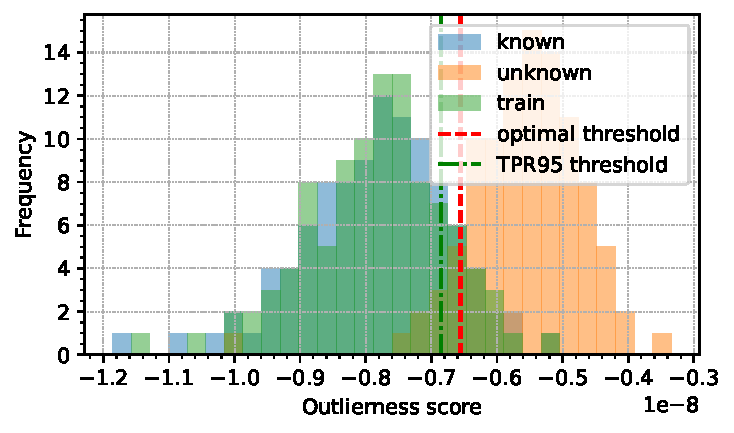
\includegraphics[width=\textwidth]{images/distributions/histograms/hist-distributions-dimension_250-samples_1000-distance_8-distribution_gaussian-model_ABOF-seed_0.pdf}
        \label{fig:histogram-abof}
    \end{subfigure}
    \hfill
    \begin{subfigure}[b]{0.495\textwidth}
        \centering
        \caption{\small Euclidean distance}
        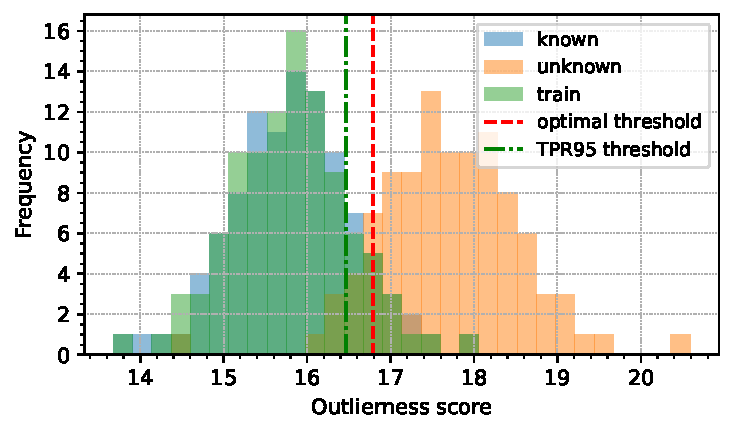
\includegraphics[width=\textwidth]{images/distributions/histograms/hist-distributions-dimension_250-samples_1000-distance_8-distribution_gaussian-model_ED-seed_0.pdf}
        \label{fig:histogram-euclidean}
    \end{subfigure}
    \begin{subfigure}[b]{0.495\textwidth}
        \centering
        \caption{\footnotesize Integrated Rank Weighted Depth ({\scriptsize$n_{proj} = 10^3$})}
        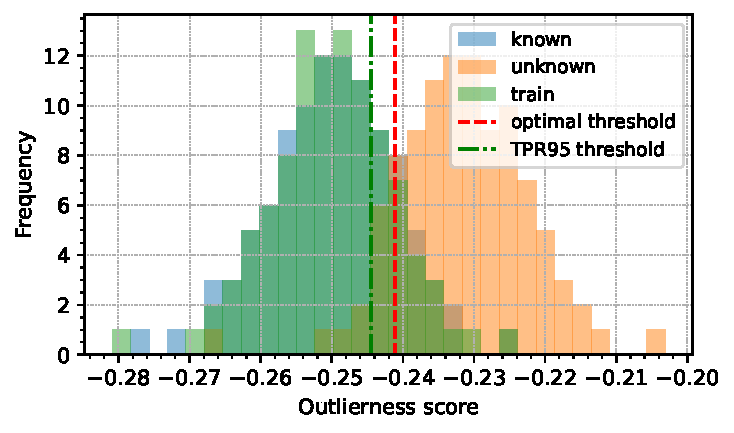
\includegraphics[width=\textwidth]{images/distributions/histograms/hist-distributions-dimension_250-samples_1000-distance_8-distribution_gaussian-model_IRWD-1000-seed_0.pdf}
        \label{fig:histogram-irwd}
    \end{subfigure}
    \hfill
    \begin{subfigure}[b]{0.495\textwidth}
        \centering
        \caption{\small k-Nearest Neighbors ($k=10$)}
        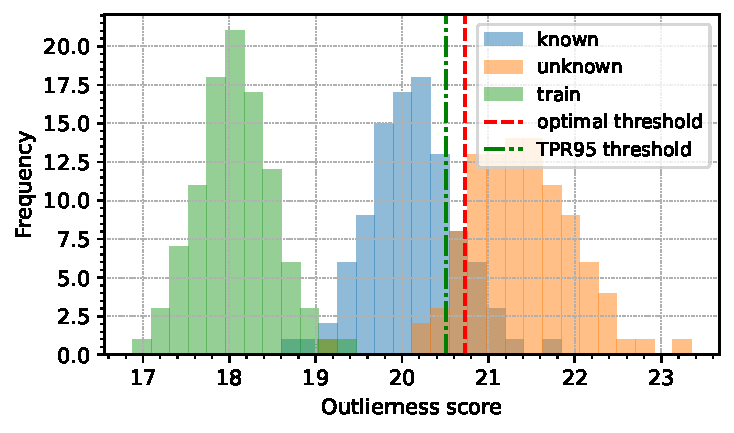
\includegraphics[width=\textwidth]{images/distributions/histograms/hist-distributions-dimension_250-samples_1000-distance_8-distribution_gaussian-model_kNN-10-seed_0.pdf}
        \label{fig:histogram-knn}
    \end{subfigure}
    \begin{subfigure}[b]{0.495\textwidth}
        \centering
        \caption{\small Local Outlier Factor ($k=10$)}
        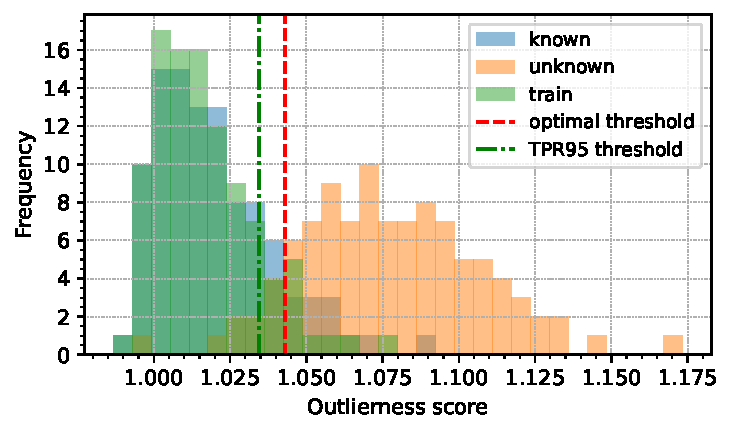
\includegraphics[width=\textwidth]{images/distributions/histograms/hist-distributions-dimension_250-samples_1000-distance_8-distribution_gaussian-model_LOF-10-seed_0.pdf}
        \label{fig:histogram-lof}
    \end{subfigure}
    \hfill
    \begin{subfigure}[b]{0.495\textwidth}
        \centering
        \caption{\small Mahalanobis distance}
        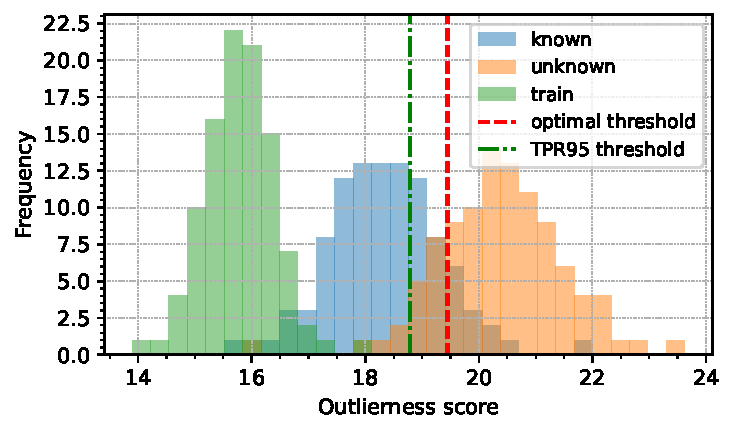
\includegraphics[width=\textwidth]{images/distributions/histograms/hist-distributions-dimension_250-samples_1000-distance_8-distribution_gaussian-model_MD-seed_0.pdf}
        \label{fig:histogram-mahalanobis}
    \end{subfigure}
    \caption{The distributions of outlierness scores obtained for various $OF$ measures (ABOF, ED, IRWD, kNN, LOF, MD). For all cases the same configuration of $T$, $K$ and $U$ clusters is~used – containing $n = 1000$ training samples, dimension of feature vectors $d = 250$, generated from $G = \textit{Gaussian}$ distribution, seed $\xi = 0$; outliers are shifted by~distance $h = 8$. In~some cases (kNN, MD) the results obtained for $K$ are~surprisingly~distant from results obtained for $T$.}
    \label{fig:histograms}
\end{figure}

\begin{figure}[t]
    % StreamLit settings: width=9, height=2
    \centering
    \begin{subfigure}[b]{\textwidth}
        \centering
        \caption{\small Angle-Based Outlier Factor}
        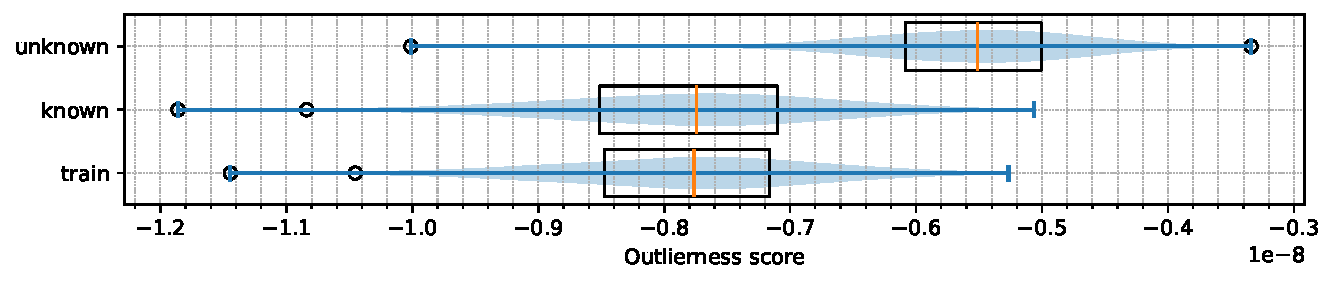
\includegraphics[width=\textwidth]{images/distributions/skew/box-distributions-dimension_250-samples_1000-distance_8-distribution_gaussian-model_ABOF-seed_0.pdf}
        \label{fig:box-abof}
    \end{subfigure}
    \begin{subfigure}[b]{\textwidth}
        \centering
        \caption{\small Euclidean distance}
        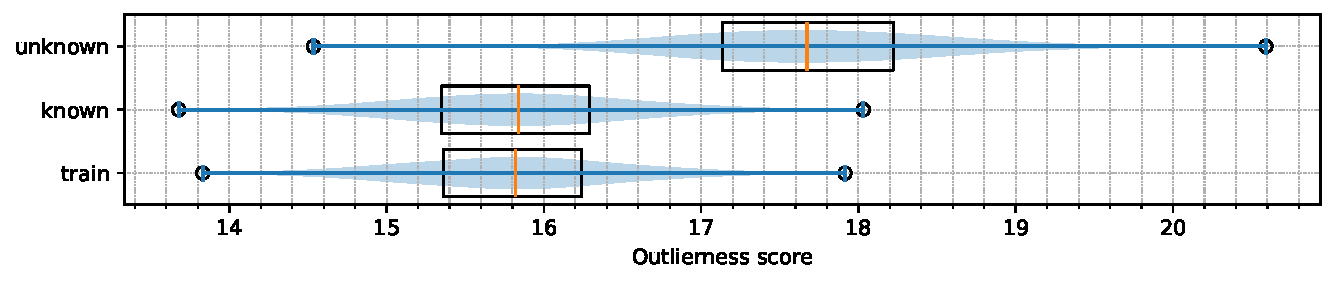
\includegraphics[width=\textwidth]{images/distributions/skew/box-distributions-dimension_250-samples_1000-distance_8-distribution_gaussian-model_ED-seed_0.pdf}
        \label{fig:box-ed}
    \end{subfigure}
    \begin{subfigure}[b]{\textwidth}
        \centering
        \caption{\small k-Nearest Neighbors ($k=10$)}
        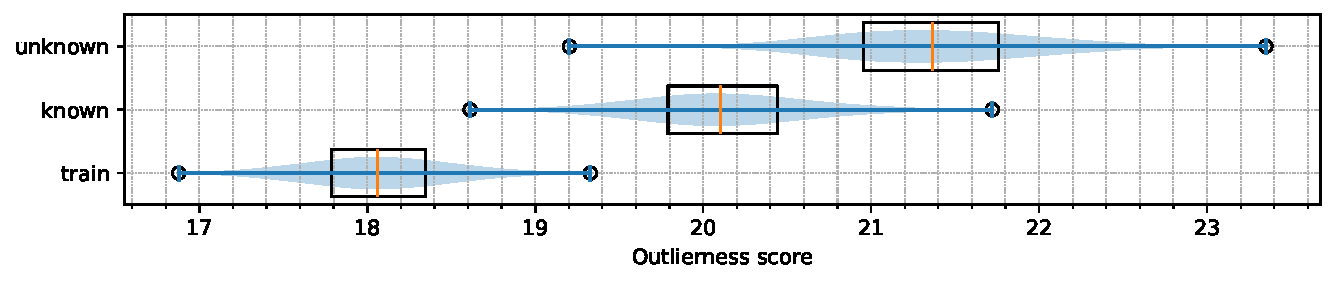
\includegraphics[width=\textwidth]{images/distributions/skew/box-distributions-dimension_250-samples_1000-distance_8-distribution_gaussian-model_kNN-10-seed_0.pdf}
        \label{fig:box-knn}
    \end{subfigure}
    \begin{subfigure}[b]{\textwidth}
        \centering
        \caption{\small Local Outlier Factor ($k=10$)}
        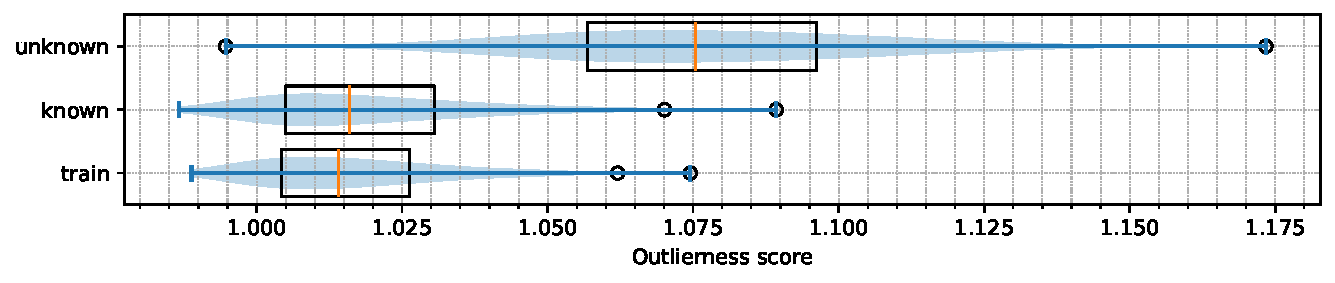
\includegraphics[width=\textwidth]{images/distributions/skew/box-distributions-dimension_250-samples_1000-distance_8-distribution_gaussian-model_LOF-10-seed_0.pdf}
        \label{fig:box-lof}
    \end{subfigure}
    \caption{The boxplots of scores distributions obtained for selected $OF$ measures (ABOF, ED, kNN, LOF) calculated on $T$, $K$ and $U$ clusters – corresponding with selected histograms from the figure \ref{fig:histograms}. The positive skew is observed in case of LOF and negative skew in case of ABOF measure, while ED and kNN appear symmetric.}
    \label{fig:boxplots}
\end{figure}

\begin{figure}[t]
    % StreamLit settings: width=5, height=3
    \centering
    \begin{subfigure}[b]{0.495\textwidth}
        \centering
        \caption{\small k-Nearest Neighbors, $G = \textit{Gaussian}$}
        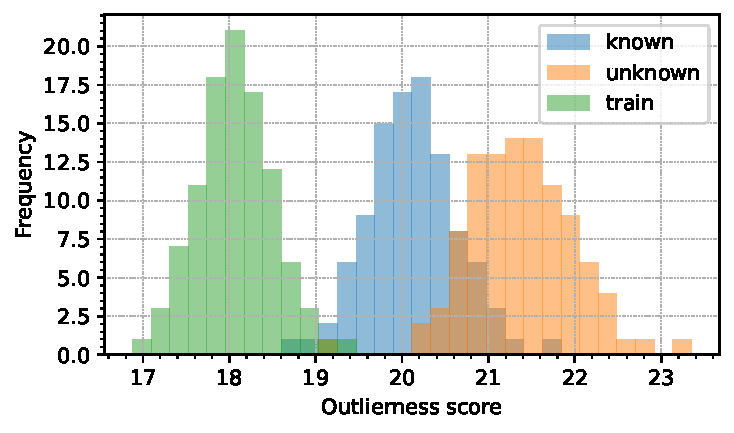
\includegraphics[width=\textwidth]{images/distributions/hists-Gen/hist-distributions-dimension_250-samples_1000-distance_8-distribution_gaussian-model_kNN-10-seed_0.pdf}
        \label{fig:hists-knn-gaussian}
    \end{subfigure}
    \hfill
    \begin{subfigure}[b]{0.495\textwidth}
        \centering
        \caption{\small Mahalanobis distance, $G = \textit{Gaussian}$}
        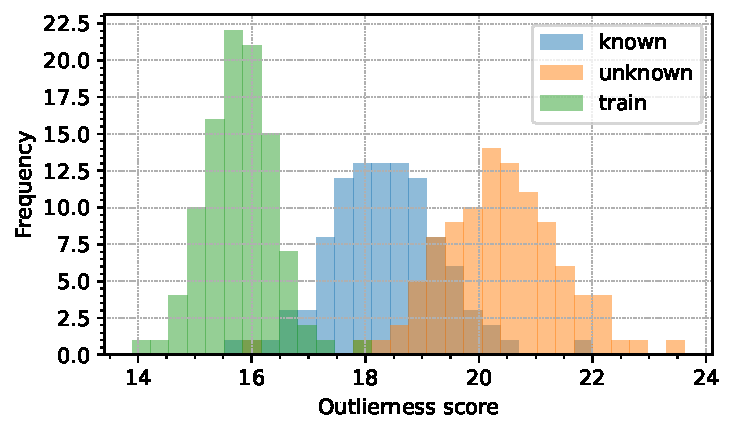
\includegraphics[width=\textwidth]{images/distributions/hists-Gen/hist-distributions-dimension_250-samples_1000-distance_8-distribution_gaussian-model_MD-seed_0.pdf}
        \label{fig:hists-md-gaussian}
    \end{subfigure}
    \begin{subfigure}[b]{0.495\textwidth}
        \centering
        \caption{\small k-Nearest Neighbors, $G = \textit{Triangular}$}
        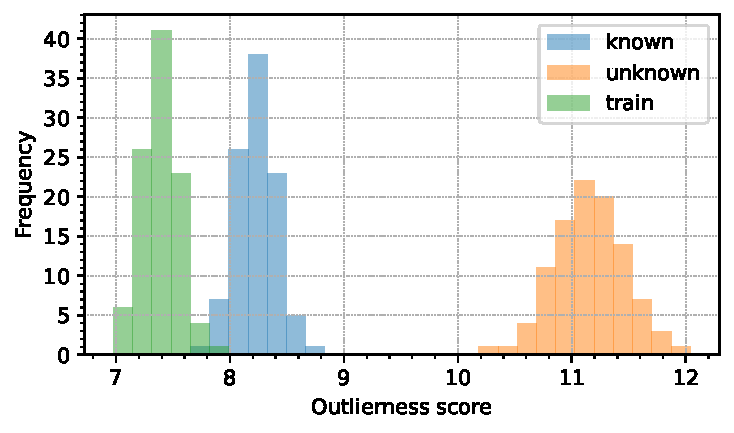
\includegraphics[width=\textwidth]{images/distributions/hists-Gen/hist-distributions-dimension_250-samples_1000-distance_8-distribution_triangular-model_kNN-10-seed_0.pdf}
        \label{fig:hists-knn-triangular}
    \end{subfigure}
    \hfill
    \begin{subfigure}[b]{0.495\textwidth}
        \centering
        \caption{\small Mahalanobis distance, $G = \textit{Triangular}$}
        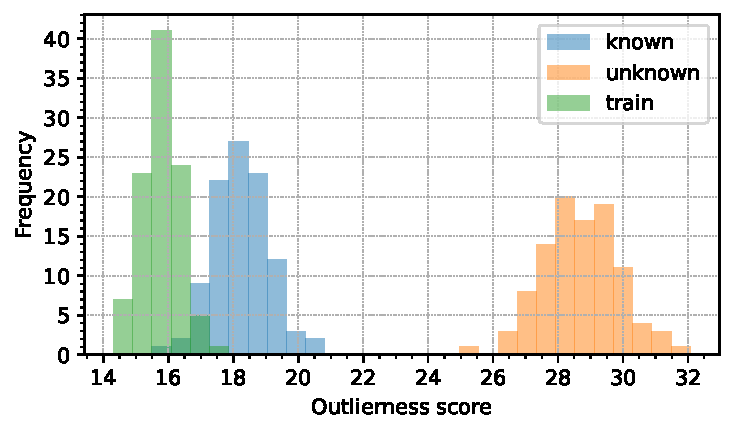
\includegraphics[width=\textwidth]{images/distributions/hists-Gen/hist-distributions-dimension_250-samples_1000-distance_8-distribution_triangular-model_MD-seed_0.pdf}
        \label{fig:hists-md-triangular}
    \end{subfigure}
    \begin{subfigure}[b]{0.495\textwidth}
        \centering
        \caption{\small k-Nearest Neighbors, $G = \textit{Uniform}$}
        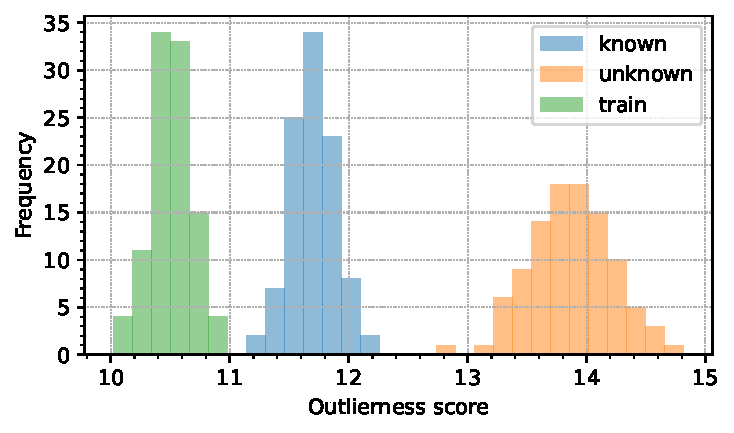
\includegraphics[width=\textwidth]{images/distributions/hists-Gen/hist-distributions-dimension_250-samples_1000-distance_8-distribution_uniform-model_kNN-10-seed_0.pdf}
        \label{fig:hists-knn-uniform}
    \end{subfigure}
    \hfill
    \begin{subfigure}[b]{0.495\textwidth}
        \centering
        \caption{\small Mahalanobis distance, $G = \textit{Uniform}$}
        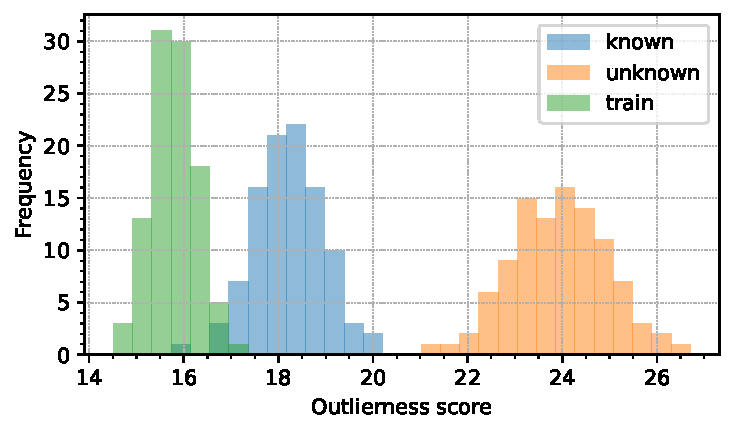
\includegraphics[width=\textwidth]{images/distributions/hists-Gen/hist-distributions-dimension_250-samples_1000-distance_8-distribution_uniform-model_MD-seed_0.pdf}
        \label{fig:hists-md-uniform}
    \end{subfigure}
    \caption{In case of kNN and MD, for high-dimensional feature vectors, the scores for known in-distribution data (cluster $K$) may not overlap with the scores obtained for the training samples (cluster $T$). This phenomenon is observed regardless of~chosen data distribution generator $G$: $\textit{Triangular}$ (shown in figures \ref{fig:hists-knn-triangular} and \ref{fig:hists-md-triangular}) or $\textit{Uniform}$ (figures \ref{fig:hists-knn-uniform} and \ref{fig:hists-md-uniform}) $\textit{Gaussian}$ (figures \ref{fig:histogram-knn} and \ref{fig:histogram-mahalanobis}). Other parameters are the same as for figure \ref{fig:histograms}: $n = 1000$, $d = 250$, $h = 8$, $\xi = 0$.}
    \label{fig:histograms-other-G}
\end{figure}

\begin{figure}[t]
    % StreamLit settings: width=9, height=2
    % Query: model = "MD" and dimension == 250 and 500 <= samples <= 5000 and distance == 8 and seed = 0 and distribution == "uniform"
    \centering
    \begin{subfigure}[b]{\textwidth}
        \centering
        \caption{\small Mahalanobis distance, training samples: $n = 500$}
        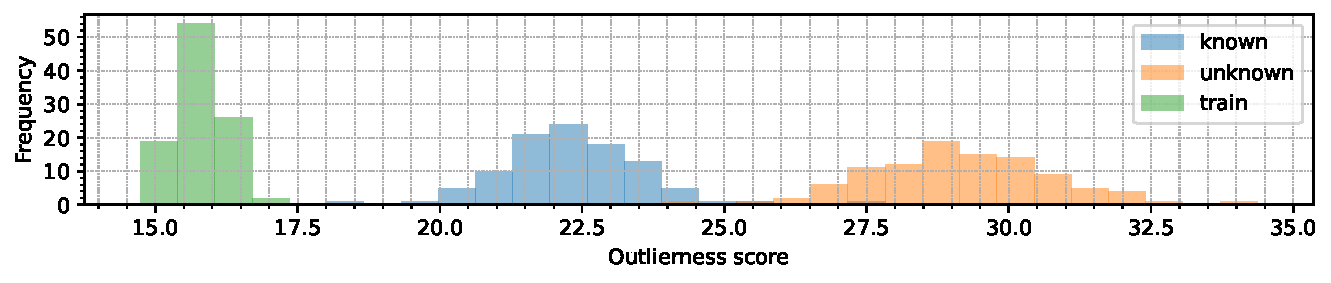
\includegraphics[width=\textwidth]{images/distributions/hists-md-samples/hist-distributions-dimension_250-samples_500-distance_8-distribution_uniform-model_MD-seed_0.pdf}
        \label{fig:hists-md-500}
    \end{subfigure}
    \begin{subfigure}[b]{\textwidth}
        \centering
        \caption{\small Mahalanobis distance, training samples: $n = 1000$}
        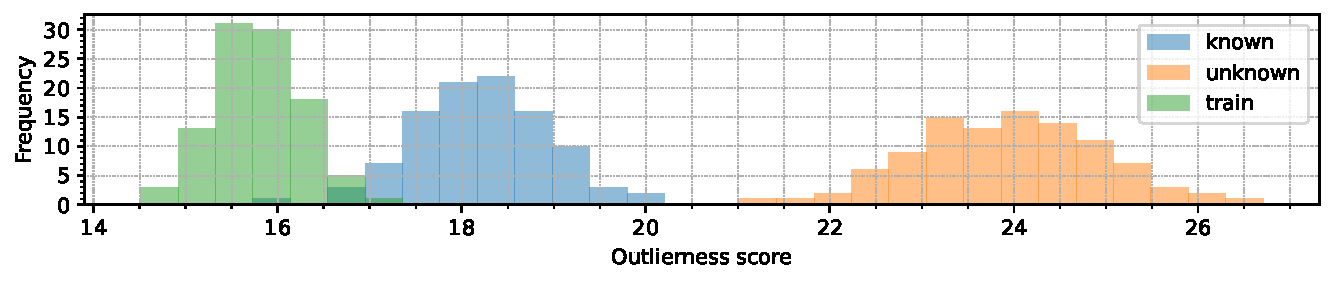
\includegraphics[width=\textwidth]{images/distributions/hists-md-samples/hist-distributions-dimension_250-samples_1000-distance_8-distribution_uniform-model_MD-seed_0.pdf}
        \label{fig:hists-md-1000}
    \end{subfigure}
    \begin{subfigure}[b]{\textwidth}
        \centering
        \caption{\small Mahalanobis distance, training samples: $n = 2500$}
        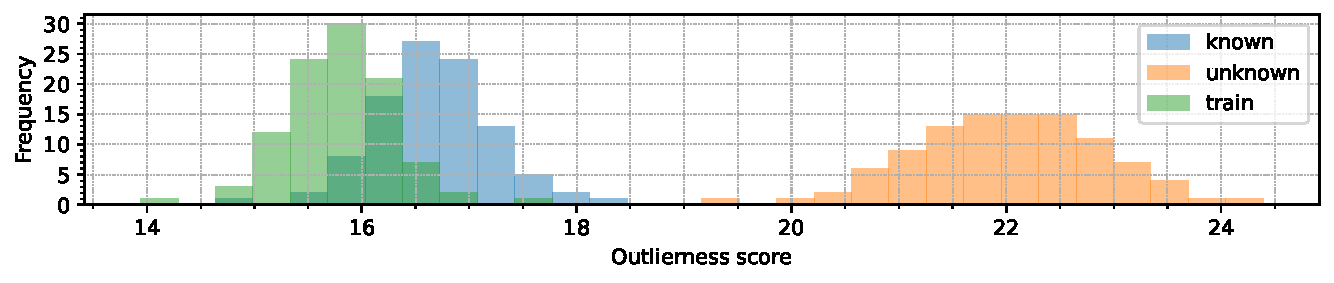
\includegraphics[width=\textwidth]{images/distributions/hists-md-samples/hist-distributions-dimension_250-samples_2500-distance_8-distribution_uniform-model_MD-seed_0.pdf}
        \label{fig:hists-md-2500}
    \end{subfigure}
    \begin{subfigure}[b]{\textwidth}
        \centering
        \caption{\small Mahalanobis distance, training samples: $n = 5000$}
        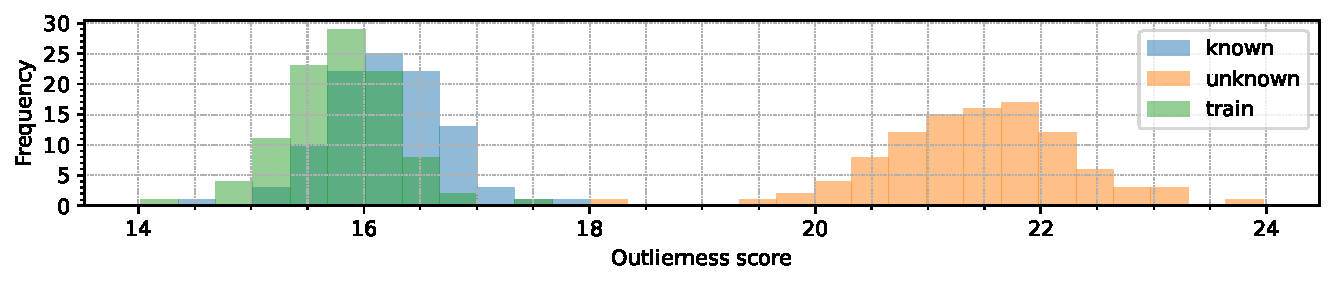
\includegraphics[width=\textwidth]{images/distributions/hists-md-samples/hist-distributions-dimension_250-samples_5000-distance_8-distribution_uniform-model_MD-seed_0.pdf}
        \label{fig:hists-md-5000}
    \end{subfigure}
    \caption{The distance between scores for known data (in-distribution, cluster $K$) and training examples (cluster $T$) gets smaller for MD when the training cluster $T$ contains more elements (parameter $n$). Note that the outliers (unknown examples, cluster $U$) are also moving closer to~$T$ (distances between medians $Q2_{T}$ and $Q2_{U}$: $\Delta{Q}_{n=500} \approx 13.31$ $\rightarrow$ $\Delta{Q}_{n=1000} \approx 8.19$ $\rightarrow$ $\Delta{Q}_{n=2500} \approx 6.22$ $\rightarrow$ $\Delta{Q}_{n=5000} \approx 5.68$), \\
    up to a~certain point –~when $K$ overlaps with $T$, then cluster $U$ no longer moves towards cluster $T$. Other distribution parameters involved: \\
    $d = 250$, $h = 8$, $G = \textit{Uniform}$, $\xi = 0$.}
    \label{fig:hists-md-samples}
\end{figure}

\begin{figure}[t]
    % StreamLit settings: width=9, height=2
    \centering
    \begin{subfigure}[b]{\textwidth}
        \centering
        \caption{\small k-Nearest Neighbors ($k=10$), training samples: $n = 500$}
        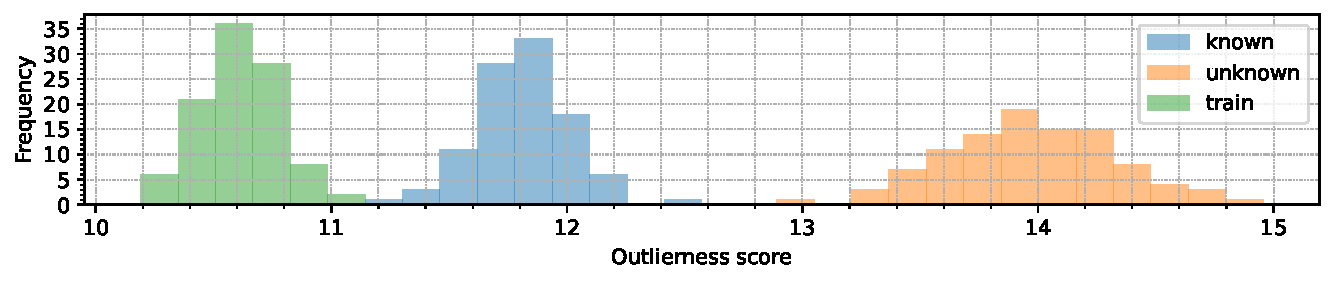
\includegraphics[width=\textwidth]{images/distributions/hists-knn-samples/hist-distributions-dimension_250-samples_500-distance_8-distribution_uniform-model_kNN-10-seed_0.pdf}
        \label{fig:hists-knn-500}
    \end{subfigure}
    \begin{subfigure}[b]{\textwidth}
        \centering
        \caption{\small k-Nearest Neighbors ($k=10$), training samples: $n = 1000$}
        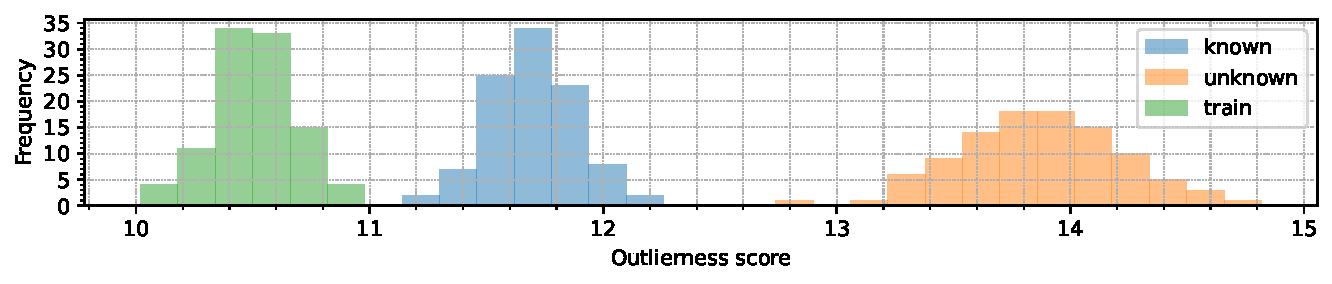
\includegraphics[width=\textwidth]{images/distributions/hists-knn-samples/hist-distributions-dimension_250-samples_1000-distance_8-distribution_uniform-model_kNN-10-seed_0.pdf}
        \label{fig:hists-knn-1000}
    \end{subfigure}
    \begin{subfigure}[b]{\textwidth}
        \centering
        \caption{\small k-Nearest Neighbors ($k=10$), training samples: $n = 5000$}
        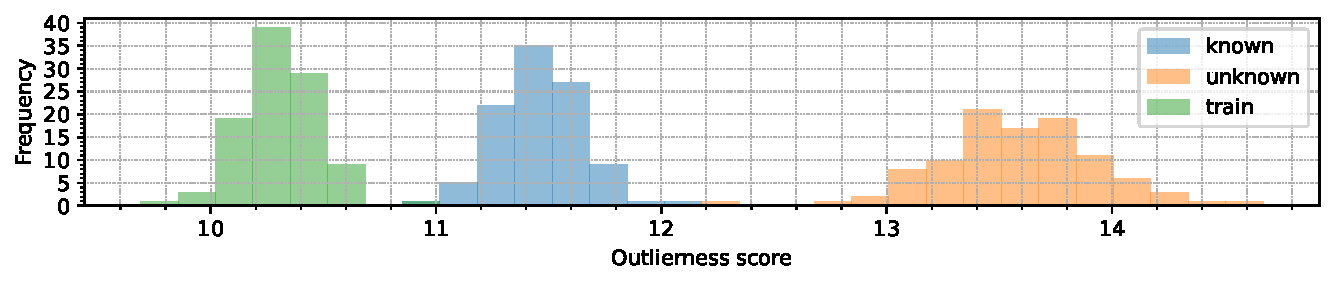
\includegraphics[width=\textwidth]{images/distributions/hists-knn-samples/hist-distributions-dimension_250-samples_5000-distance_8-distribution_uniform-model_kNN-10-seed_0.pdf}
        \label{fig:hists-knn-5000}
    \end{subfigure}
    \begin{subfigure}[b]{\textwidth}
        \centering
        \caption{\small k-Nearest Neighbors ($k=20$), training samples: $n = 1000$}
        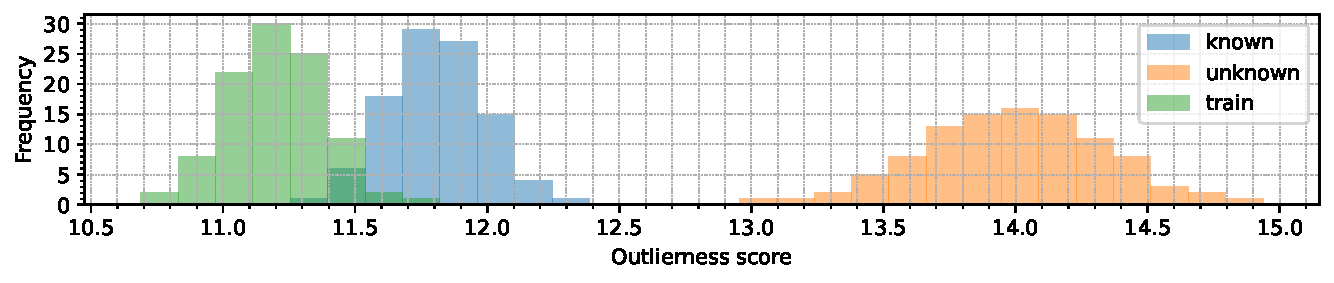
\includegraphics[width=\textwidth]{images/distributions/hists-knn-samples/hist-distributions-dimension_250-samples_1000-distance_8-distribution_uniform-model_kNN-20-seed_0.pdf}
        \label{fig:hists-knn20-1000}
    \end{subfigure}
    \caption{Unlike for MD, increasing the number of training samples $n$ in cluster $T$ does not bring the cluster $K$ scores significantly closer to scores for cluster $T$. Scores obtained for outliers (cluster $U$) also remain unaffected by $n$. However, the results for~$K$ and $T$ start to overlap for larger values of $k$ (parameter of kNN algorithm). Experiment settings are the same as in figure \ref{fig:hists-md-samples} ({\small$d = 250$, $h = 8$, $G = \textit{Uniform}$, $\xi = 0$}).}
    \label{fig:hists-knn-samples}
\end{figure}

\begin{figure}[t]
    % StreamLit settings: width=9, height=2
    \centering
    \begin{subfigure}[b]{\textwidth}
        \centering
        \caption{\small k-Nearest Neighbors ($k=10$), dimension of feature vectors: $d = 100$}
        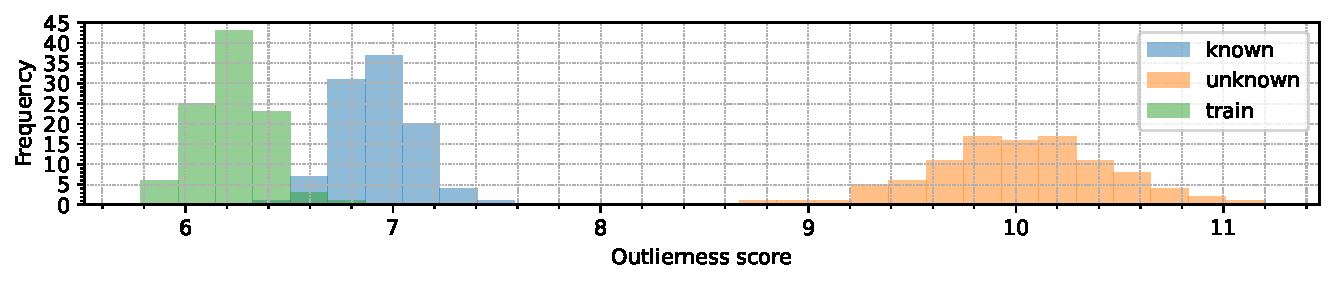
\includegraphics[width=\textwidth]{images/distributions/hists-dimensions/hist-distributions-dimension_100-samples_1000-distance_8-distribution_uniform-model_kNN-10-seed_0.pdf}
        \label{fig:hists-knn-d100}
    \end{subfigure}
    \begin{subfigure}[b]{\textwidth}
        \centering
        \caption{\small k-Nearest Neighbors ($k=10$), dimension of feature vectors: $d = 500$}
        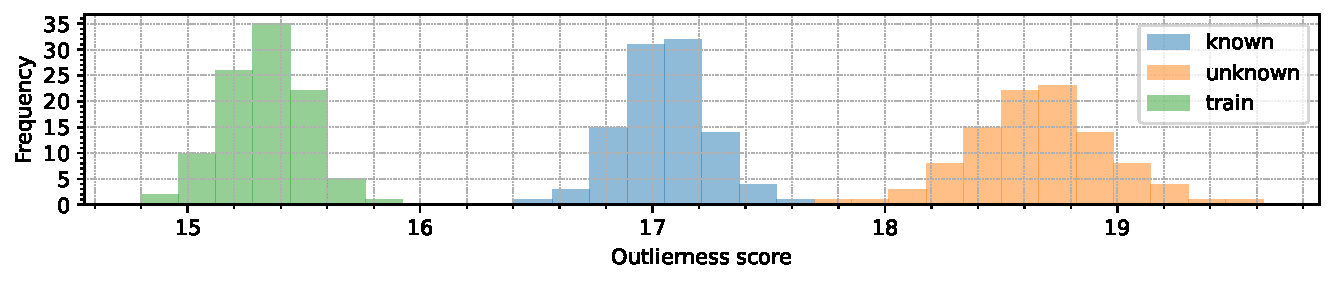
\includegraphics[width=\textwidth]{images/distributions/hists-dimensions/hist-distributions-dimension_500-samples_1000-distance_8-distribution_uniform-model_kNN-10-seed_0.pdf}
        \label{fig:hists-knn-d500}
    \end{subfigure}
    \begin{subfigure}[b]{\textwidth}
        \centering
        \caption{\small Mahalanobis distance, dimension of feature vectors: $d = 100$}
        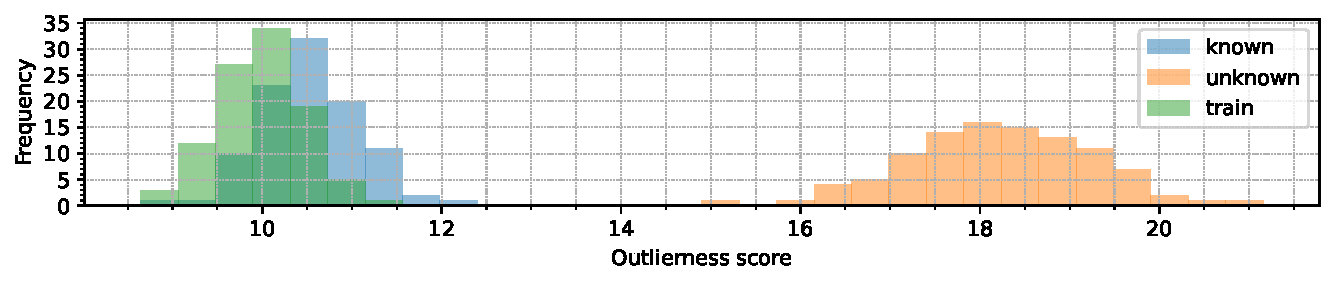
\includegraphics[width=\textwidth]{images/distributions/hists-dimensions/hist-distributions-dimension_100-samples_1000-distance_8-distribution_uniform-model_MD-seed_0.pdf}
        \label{fig:hists-md-d100}
    \end{subfigure}
    \begin{subfigure}[b]{\textwidth}
        \centering
        \caption{\small Mahalanobis distance, dimension of feature vectors: $d = 500$}
        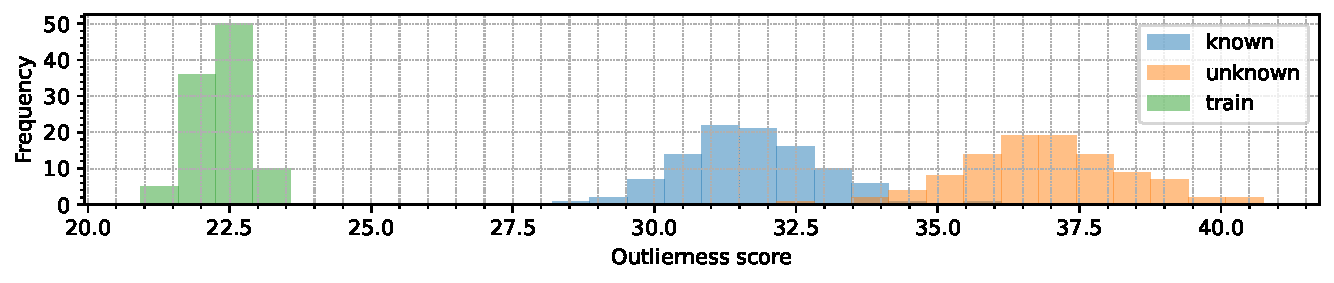
\includegraphics[width=\textwidth]{images/distributions/hists-dimensions/hist-distributions-dimension_500-samples_1000-distance_8-distribution_uniform-model_MD-seed_0.pdf}
        \label{fig:hists-md-d500}
    \end{subfigure}
    \caption{The effect of distancing scores acquired for cluster $K$ from the scores obtained for cluster $T$, observed in case of kNN and MD measures, is stronger for increased dimensionality of feature vectors $d$. It can be noticed that for higher dimensions the scores values are also greater, as both the measures are based on spatial distances in features space, hence more feature vectors components contribute to~greater score values. Results visible in plots are obtained for experiment settings: $n = 1000$, $h = 8$, $G = \textit{Uniform}$, $\xi = 0$.}
    \label{fig:hists-dimensions}
\end{figure}

\begin{figure}[tb]
    \vspace{-2.0em}
    % StreamLit settings: width=9, height=2
    \centering
    \begin{subfigure}[b]{\textwidth}
        \centering
        \caption{\small Standardized Euclidean distance, dimension of feature vectors: $d = 100$}
        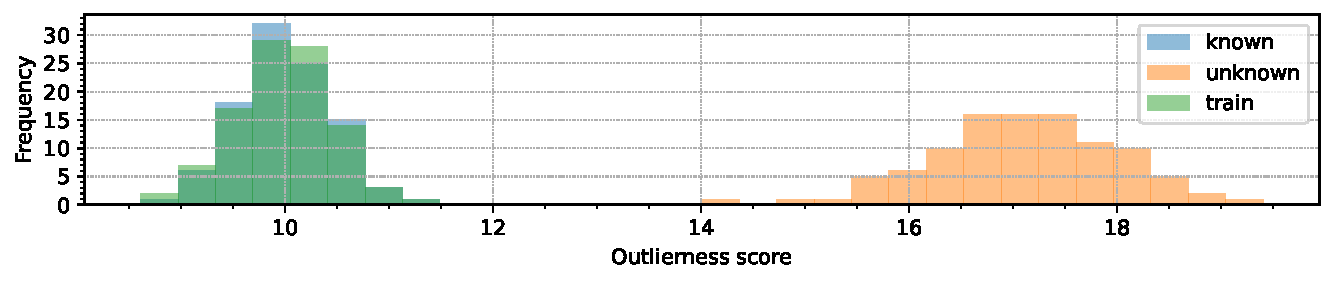
\includegraphics[width=\textwidth]{images/distributions/hists-sed-dimensions/hist-distributions-dimension_100-samples_1000-distance_8-distribution_uniform-model_SED-seed_0.pdf}
        \label{fig:hists-sed-100}
    \end{subfigure}
    \begin{subfigure}[b]{\textwidth}
        \centering
        \caption{\small Standardized Euclidean distance, dimension of feature vectors: $d = 500$}
        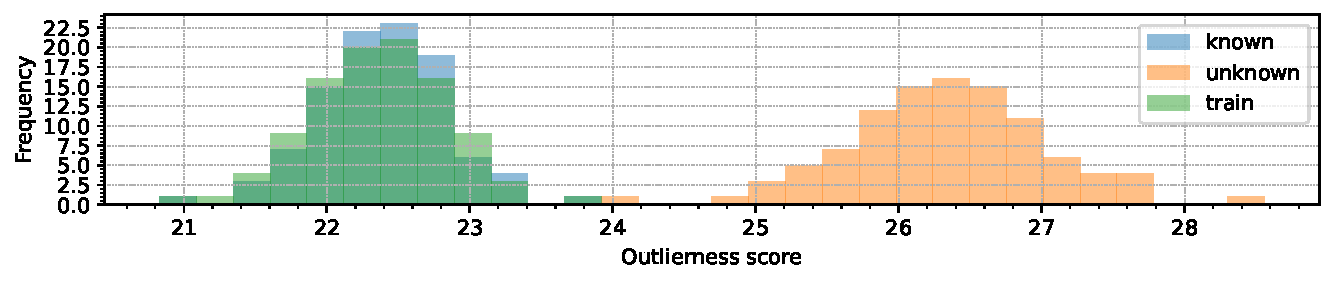
\includegraphics[width=\textwidth]{images/distributions/hists-sed-dimensions/hist-distributions-dimension_500-samples_1000-distance_8-distribution_uniform-model_SED-seed_0.pdf}
        \label{fig:hists-sed-500}
    \end{subfigure}
    \caption{For measures ABOF, IRWD, LOF, ED and SED, in typical conditions, $n \gtrsim d$, the separation between scores for in-distribution data (cluster $K$ and cluster $T$) is not observed, maintaining good overlapping even for a lower number of training samples $n$ than for MD. Experiment settings: $n = 1000$, $h = 8$, $G = \textit{Uniform}$, $\xi = 0$.}
    \label{fig:hists-sed-dimensions}
\end{figure}
\begin{figure}[tb]
    \vspace{-1.0em}
    % StreamLit settings: width=9, height=2
    \centering
    \begin{subfigure}[b]{\textwidth}
        \centering
        \caption{\small Angle-Based Outlier Factor, dimension: $d = 1000$, samples: $n = 50$}
        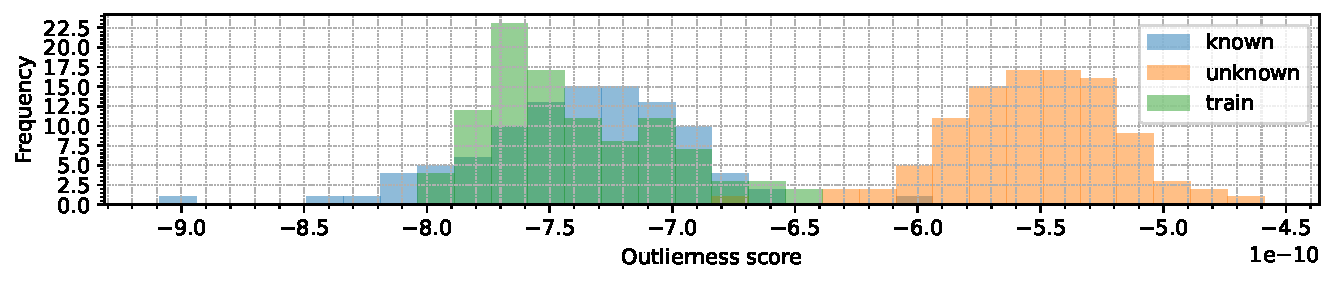
\includegraphics[width=\textwidth]{images/distributions/hists-extreme/hist-distributions-dimension_1000-samples_50-distance_8-distribution_uniform-model_ABOF-seed_0.pdf}
        \label{fig:hists-abof-n50}
    \end{subfigure}
    \begin{subfigure}[b]{\textwidth}
        \centering
        \caption{\small Local Outlier Factor ($k=10$), dimension: $d = 1000$, samples: $n = 50$}
        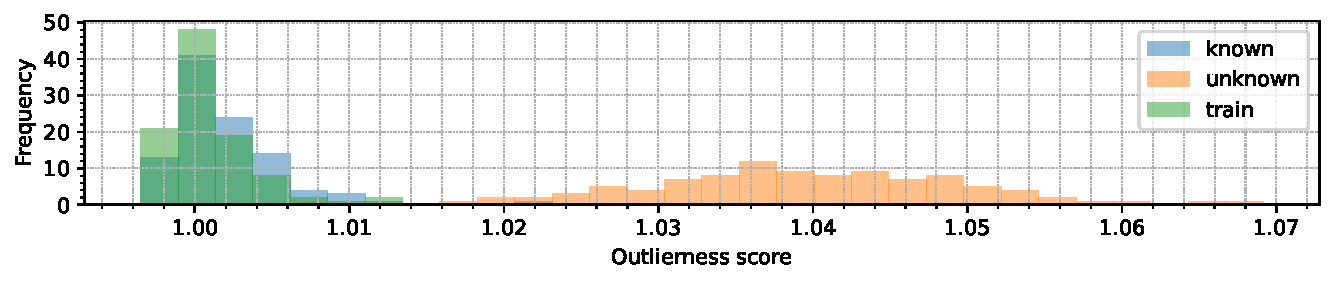
\includegraphics[width=\textwidth]{images/distributions/hists-extreme/hist-distributions-dimension_1000-samples_50-distance_8-distribution_uniform-model_LOF-10-seed_0.pdf}
        \label{fig:hists-lof-n50}
    \end{subfigure}
    \caption{In the performed study, ABOF and LOF were able to produce accurate representations even in case of significantly under-represented testing cluster –~obtained scores for $T$ and $K$ do overlap despite $n = 50$ training samples for $d = 1000$ dimension of feature vectors. Remaining experiment settings are: $h = 8$, $G = \textit{Uniform}$, $\xi = 0$.}
    \label{fig:hists-extreme-good}
    \vspace{-3.0em}
\end{figure}

\begin{figure}[t]
    % StreamLit settings: width=9, height=2
    \centering
    \begin{subfigure}[b]{\textwidth}
        \centering
        \caption{\small Integrated Rank Weighted Depth ({\scriptsize$n_{proj} = 10^3$}), dimension: $d = 500$, samples: $n = 50$}
        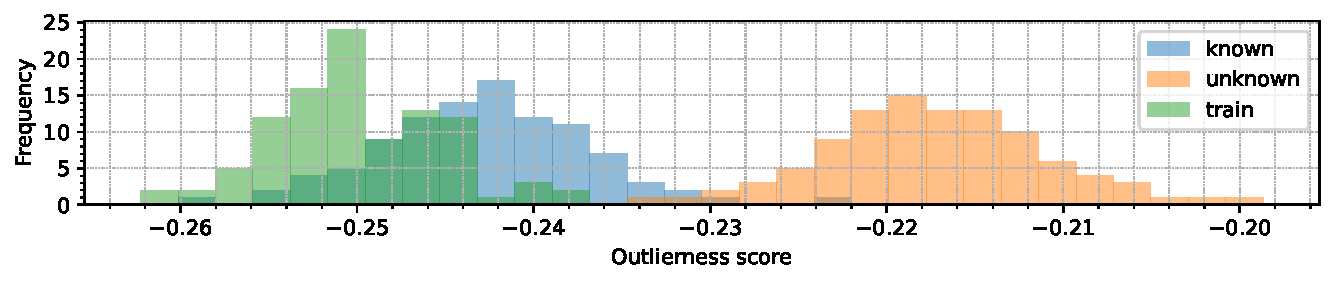
\includegraphics[width=\textwidth]{images/distributions/hists-extreme/hist-distributions-dimension_500-samples_50-distance_8-distribution_uniform-model_IRWD-1000-seed_0.pdf}
        \label{fig:hists-irwd-n50}
    \end{subfigure}
    \begin{subfigure}[b]{\textwidth}
        \centering
        \caption{\small Integrated Rank Weighted Depth ({\scriptsize$n_{proj} = 10^3$}), dimension: $d = 500$, samples: $n = 500$}
        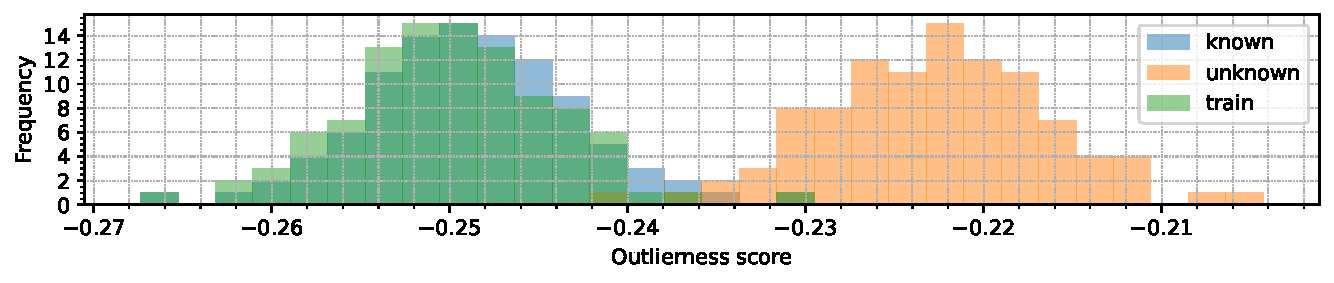
\includegraphics[width=\textwidth]{images/distributions/hists-extreme/hist-distributions-dimension_500-samples_500-distance_8-distribution_uniform-model_IRWD-1000-seed_0.pdf}
        \label{fig:hists-irwd-n500}
    \end{subfigure}
    \begin{subfigure}[b]{\textwidth}
        \centering
        \caption{\small Standardized Euclidean distance, dimension: $d = 1000$, training samples: $n = 50$}
        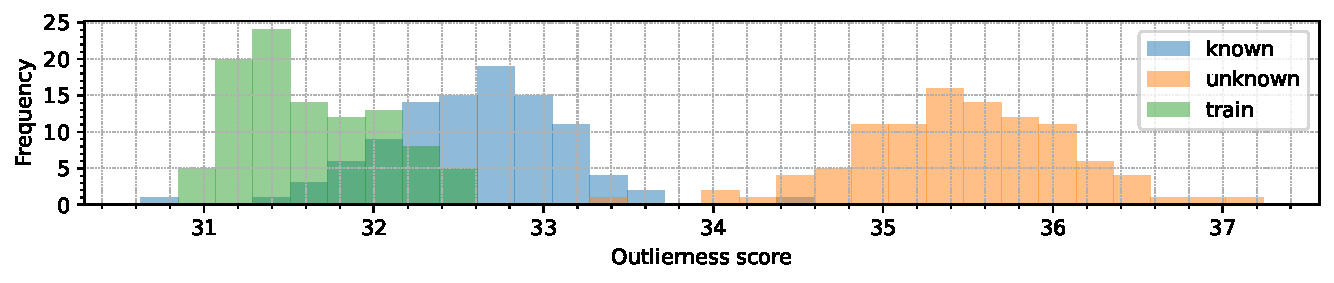
\includegraphics[width=\textwidth]{images/distributions/hists-extreme/hist-distributions-dimension_1000-samples_50-distance_8-distribution_uniform-model_SED-seed_0.pdf}
        \label{fig:hists-sed-n50}
    \end{subfigure}
    \begin{subfigure}[b]{\textwidth}
        \centering
        \caption{\small Standardized Euclidean distance, dimension: $d = 1000$, training samples: $n = 1000$}
        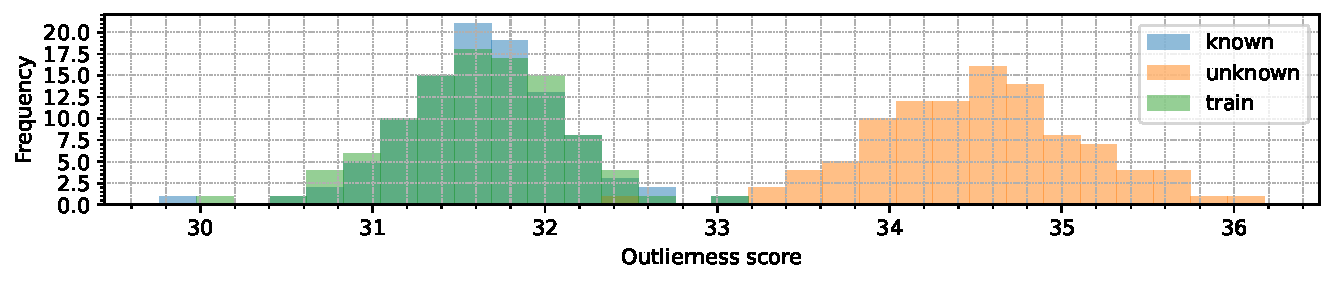
\includegraphics[width=\textwidth]{images/distributions/hists-extreme/hist-distributions-dimension_1000-samples_1000-distance_8-distribution_uniform-model_SED-seed_0.pdf}
        \label{fig:hists-sed-n1000}
    \end{subfigure}
    \caption{For strongly under-represented training clusters, $n \ll d$, the effect of~not-overlapping between the scores for cluster $T$ and $K$ is observed in case of~IRWD, ED and SED measures. The effect vanishes when $n$ is not so low, yet it does not need to be as big as for MD to reach overlapping (settings: $h = 8$, $G = \textit{Uniform}$, $\xi = 0$).}
    \label{fig:hists-extreme-bad}
\end{figure}

\begin{figure}[t]
    % StreamLit settings: width=5, height=3
    \centering
    \begin{subfigure}[b]{0.495\textwidth}
        \centering
        \caption{\small Angle-Based Outlier Factor}
        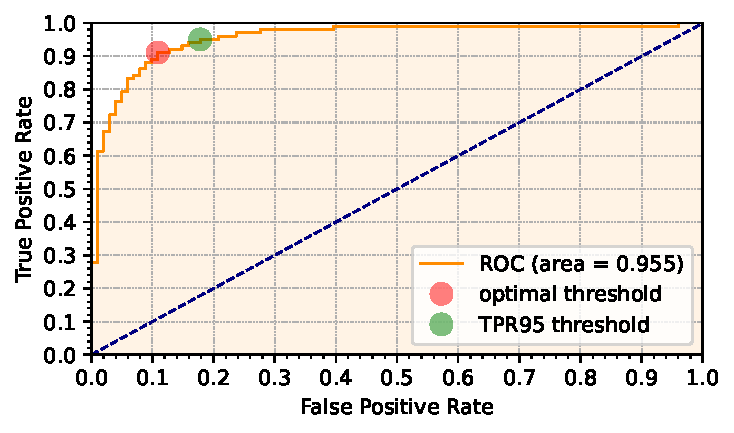
\includegraphics[width=\textwidth]{images/distributions/rocs/roc-distributions-dimension_250-samples_1000-distance_8-distribution_gaussian-model_ABOF-seed_0.pdf}
        \label{fig:roc-abof}
    \end{subfigure}
    \hfill
    \begin{subfigure}[b]{0.495\textwidth}
        \centering
        \caption{\small Euclidean distance}
        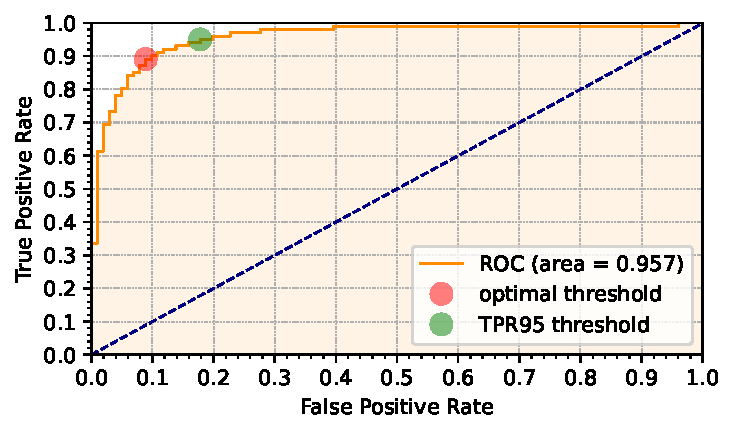
\includegraphics[width=\textwidth]{images/distributions/rocs/roc-distributions-dimension_250-samples_1000-distance_8-distribution_gaussian-model_ED-seed_0.pdf}
        \label{fig:roc-euclidean}
    \end{subfigure}
    \begin{subfigure}[b]{0.495\textwidth}
        \centering
        \caption{\footnotesize Integrated Rank Weighted Depth ({\scriptsize$n_{proj} = 10^3$})}
        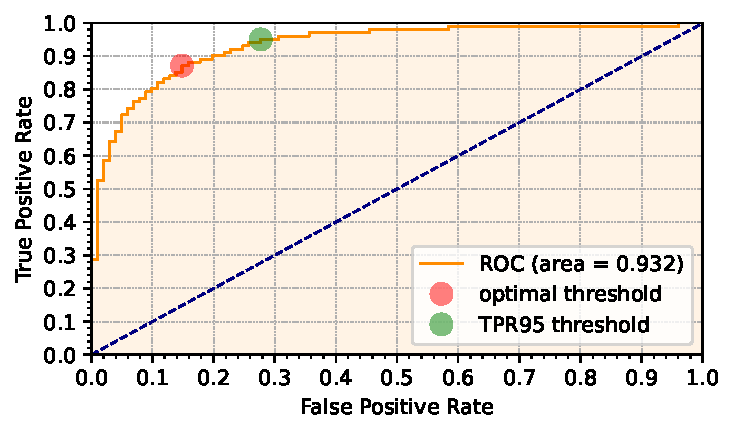
\includegraphics[width=\textwidth]{images/distributions/rocs/roc-distributions-dimension_250-samples_1000-distance_8-distribution_gaussian-model_IRWD-1000-seed_0.pdf}
        \label{fig:roc-irwd}
    \end{subfigure}
    \hfill
    \begin{subfigure}[b]{0.495\textwidth}
        \centering
        \caption{\small k-Nearest Neighbors ($k=10$)}
        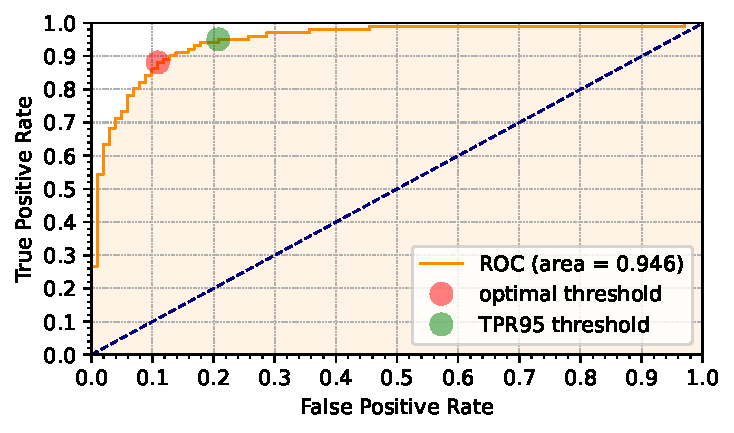
\includegraphics[width=\textwidth]{images/distributions/rocs/roc-distributions-dimension_250-samples_1000-distance_8-distribution_gaussian-model_kNN-10-seed_0.pdf}
        \label{fig:roc-knn}
    \end{subfigure}
    \begin{subfigure}[b]{0.495\textwidth}
        \centering
        \caption{\small Local Outlier Factor ($k=10$)}
        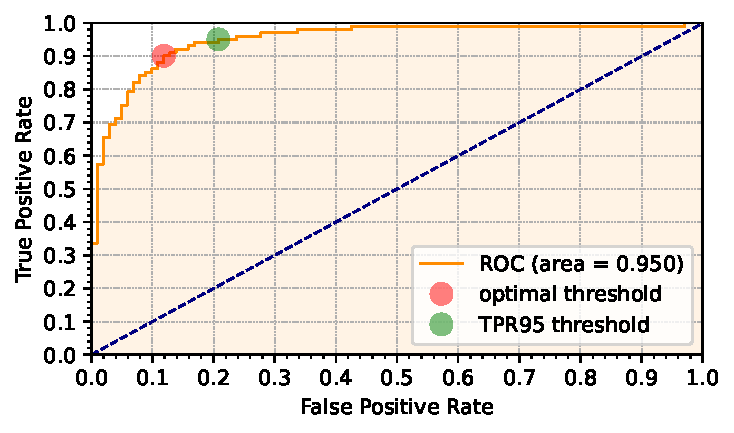
\includegraphics[width=\textwidth]{images/distributions/rocs/roc-distributions-dimension_250-samples_1000-distance_8-distribution_gaussian-model_LOF-10-seed_0.pdf}
        \label{fig:roc-lof}
    \end{subfigure}
    \hfill
    \begin{subfigure}[b]{0.495\textwidth}
        \centering
        \caption{\small Mahalanobis distance}
        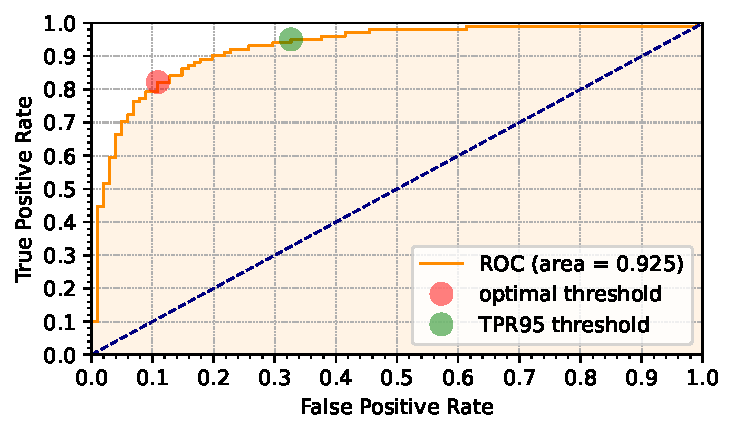
\includegraphics[width=\textwidth]{images/distributions/rocs/roc-distributions-dimension_250-samples_1000-distance_8-distribution_gaussian-model_MD-seed_0.pdf}
        \label{fig:roc-mahalanobis}
    \end{subfigure}
    \caption{The Receiver Operating Characteristic (ROC) curves obtained for various $OF$ measures (ABOF, ED, IRWD, kNN, LOF, MD). They show the sepearability between clusters $K$ and $U$ visible in corresponding plots from the~figure~\ref{fig:histograms}.
    Despite that some $OF$ methods represent $K$ as distant from $T$, they still can distinguish between $K$ and $U$ quite well, all acquiring high AUROC scores \\
    (the~area values of visible subplots are all greater than $0.9$).}
    \label{fig:rocs}
\end{figure}

\cleardoublepage{}
